\documentclass{paper}

%\usepackage{times}
\usepackage{epsfig}
\usepackage{graphicx}
\usepackage{amsmath}
\usepackage{amssymb}
\usepackage{color}
\usepackage{subcaption}




% load package with ``framed'' and ``numbered'' option.
%\usepackage[framed,numbered,autolinebreaks,useliterate]{mcode}

% something NOT relevant to the usage of the package.
\setlength{\parindent}{0pt}
\setlength{\parskip}{18pt}






\usepackage[latin1]{inputenc} 
\usepackage[T1]{fontenc} 

\usepackage{listings} 
\lstset{% 
   language=Matlab, 
   basicstyle=\small\ttfamily, 
} 



\title{Assignment 2}



\author{Simon Jenni\\09-116-005}
% //////////////////////////////////////////////////

\AtBeginDocument{
  \let\div\relax
  \DeclareMathOperator{\div}{div}
}

\begin{document}

\maketitle


% Add figures:
%\begin{figure}[t]
%%\begin{center}
%\quad\quad   \includegraphics[width=1\linewidth]{ass2}
%%\end{center}
%
%\label{fig:performance}
%\end{figure}

\section*{Superresolution}


\begin{enumerate}

\item \textbf{Primal-Dual formulation for superresolution.}

The primal-dual formulation of a problem
\begin{equation}\label{eq:pddef}
\min_{x\in X}F(Kx)+G(x),
\end{equation}
where $F$ and $G$ are convex functions and $K$ is a linear operator, is given by 
\begin{equation}
\min_{x\in X}\max_{y\in Y}<Kx,y>-F^*(y)+G(x),
\end{equation}
and can be obtained by applying the Legendre-Fenchel transform to $F$ in order to decouple the variables $u$. 


The original formulation of the superresolution problem is given by
\begin{equation}\label{eq:energy}
E(u)=\frac{\lambda}{2}||Du-g||^2+||\nabla u||.
\end{equation}
We observe that the variable $u$ is coupled in both terms by the linear operators $D$ and $\nabla$. 
To put equation \ref{eq:energy} into a similar form of equation \ref{eq:pddef} we can set $F_1(x)=\frac{\lambda}{2}||x-g||^2$, $F_2(x)=||x||_2$ and $G(x)=0$. To arrive at the primal-dual formulation, the Legendre-Fenchel transforms of $F_1$ and $F_2$ have to be computed. They are given by:
\begin{align*}
F_1^*(v) &= \sup_x<v,x>-F_1(v) \\
&=\sup_x<v,x>-\frac{\lambda}{2}||x-g||^2 
\end{align*}         
To compute the maximum w.r.t $x$, the derivative of the right hand side w.r.t $x$ can be set to zero:
\begin{align*}
v-\lambda(x-g) &\overset{!}{=} 0 \\
x &=\frac{v}{\lambda}+g
\end{align*}  
Plugging this back into the equation for $F_1^*$ and simplifying results in:

\begin{equation}
F_1^*(v) = \frac{1}{2\lambda}||v||_2^2+<v,g>
\end{equation}         

The transform of the $l_2$-norm has already been derived in class and is given by:
\[
F_2^*(w) = \delta(w) = 
  \begin{cases}
   0 & \text{if } ||w|| < 1 \\
   \infty       & \text{otherwise}
  \end{cases}
\]

Putting all things together and simplifying, we arrive at the following primal-dual formulation:
\begin{equation}
\min_u \max_{v,w} <Du-g,v> - \frac{1}{2\lambda}||v||_2^2 + <\nabla u,w>-\delta(w)
\end{equation}    

\begin{figure}[h]
\begin{center}
	\begin{subfigure}[b]{0.49\textwidth}
                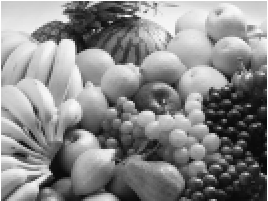
\includegraphics[width=\textwidth]{it0}
                \caption{1st Iteration}
        \end{subfigure}
        	\begin{subfigure}[b]{0.49\textwidth}
                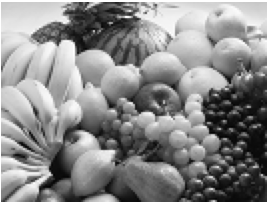
\includegraphics[width=\textwidth]{it600}
                \caption{600th Iteration}
        \end{subfigure}
        \begin{subfigure}[b]{0.49\textwidth}
                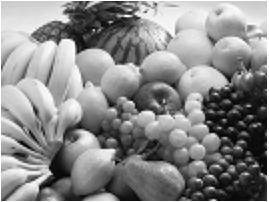
\includegraphics[width=\textwidth]{it1200}
                \caption{1200th Iteration}
        \end{subfigure}
        \begin{subfigure}[b]{0.49\textwidth}
                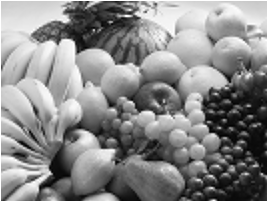
\includegraphics[width=\textwidth]{it1800}
                \caption{1800th Iteration}
        \end{subfigure}
        \begin{subfigure}[b]{0.49\textwidth}
                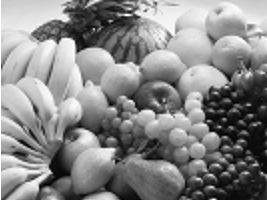
\includegraphics[width=\textwidth]{it2400}
                \caption{2400th Iteration}
        \end{subfigure}
        \begin{subfigure}[b]{0.49\textwidth}
                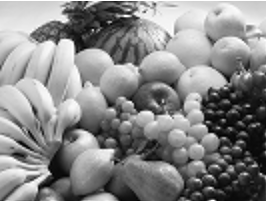
\includegraphics[width=\textwidth]{itFinal}
                \caption{Final Iteration (3000th)}
        \end{subfigure}
\end{center}
\caption{This figure shows an image at several different stages of the primal-dual algorithm. }
\label{fig:iterations}
\end{figure}

\item \textbf{Primal-Dual steps}


The primal-dual steps are defined as:
\begin{equation}
v^{n+1} = \text{prox}_{\sigma F_1^*} (v^n + \sigma D \bar{u}^n) 
\end{equation}  
\begin{equation}
w^{n+1} = \text{prox}_{\sigma F_2^*} (w^n + \sigma \nabla \bar{u}^n) 
\end{equation}   
\begin{equation}
u^{n+1} = \text{prox}_{\tau G} (u^n  - \tau D^* v^{n+1} - \tau \div w^{n+1}) 
\end{equation}   
\begin{equation}
\bar{u}^{n+1} = u^{n+1} + \theta(u^{n+1}-u^n)
\end{equation}   

Where $\div$ is the divergence operator (the adjoint of $\nabla$) and  the proximity operator $\text{prox}_{\lambda F}$ is defined by
\begin{equation}
\text{prox}_{\lambda F}(z) = \text{arg} \min_x \frac{1}{2} ||x-z||_2^2+\lambda F(x).
\end{equation}  

Using this definition, we can derive the expressions for the primal-dual steps as follows:
\begin{equation}
v^{n+1} =\text{arg} \min_x \frac{1}{2} ||x-v^n-\sigma D \bar{u}^n||_2^2 + \sigma(\frac{1}{2\lambda}||x||_2^2+<x,g>)
\end{equation}
To obtain the value of $x$ which minimises the expression on the right, we set the derivative w.r.t $x$ equal to zero,
\begin{align*}
x-v^n-\sigma D \bar{u}^n + \sigma(\frac{x}{\lambda} +g) &\overset{!}{=} 0 
\end{align*} 
which results in 

\begin{equation}
v^{n+1}=\frac{v^n+\sigma(D\bar{u}^n-g)}{(1+\frac{\sigma}{\lambda})}
\end{equation}

Similarly, the expression for $w^{n+1}$ can be obtained by:
\begin{align*}
w^{n+1} &= \text{arg} \min_x \frac{1}{2} ||x-w^n-\sigma \nabla \bar{u}^n||_2^2 + \sigma \delta(x)\\
 &= 
  \begin{cases}
   w^n+\sigma \nabla \bar{u}^n, & \text{if } ||w^n+\sigma \nabla \bar{u}^n|| \leq 1 \\
   \frac{w^n+\sigma \nabla \bar{u}^n}{||w^n+\sigma \nabla \bar{u}^n||} ,  & \text{otherwise}
  \end{cases} \\
&=\frac{w^n+\sigma \nabla \bar{u}^n}{\max(1,||w^n+\sigma \nabla \bar{u}^n||)}
\end{align*} 


Finally, the expression for $u^{n+1}$ is given by (remembering that $G(x)=0$):
\begin{align*}
u^{n+1} &= \text{arg} \min_x \frac{1}{2} ||x-u^n +\tau D^* v^{n+1} +\tau \div w^{n+1}||_2^2 \\
 &= u^n -\tau D^* v^{n+1} -\tau \div w^{n+1}
\end{align*} 

\item \textbf{Implementation of the primal-dual method.} 

Implementing the primal-dual steps, requires to choose appropriate values for the parameters $\sigma, \tau$ and $\theta$. The parameters are required to satisfy $\tau\sigma||K||^2<1$, where $K$ is the linear operator in Eq. \ref{eq:pddef}. This of course requires to know $||D||^2$ and $||\nabla||^2$. It is easy to see that $||D||^2=\frac{1}{\alpha^2}$, where $\alpha$ is the downsampling factor. For  $||\nabla||^2$ we can estimate an upper bound:
\begin{align*}
||\nabla x||^2 &= \sum_{i,j}(x_{i+1,j}-x_{i,j})^2+(x_{i,j+1}-x_{i,j})^2 \\
& \leq \sum_{i,j} 4x_{i,j}^2+2(x_{i+1,j}^2+x_{i,j+1}^2) \\
& \leq 8 \sum_{i,j} x_{i,j}^2 = 8\cdot||x||^2
\end{align*} 
Where we used $(x-y)^2\geq 0 \Rightarrow x^2+y^2 \geq 2xy$ for the first inequality. Therefore the parameters are chosen such that $\tau\sigma<1/\max(8,\frac{1}{\alpha^2})$. Experimentally I found that choosing the parameters dependant on $\lambda$ to be beneficial, concretely I would set $\tau=\lambda^{-\frac{1}{2}}$, $\sigma=\frac{1}{8\tau}$ and $\theta=1$. 

The gradient and divergence operator were implemented using forward differences and von Neumann boundary assumptions. Figure \ref{fig:iterations} shows images at different stages of the algorithm. 

\begin{figure}[t]
\begin{center}
\quad\quad
         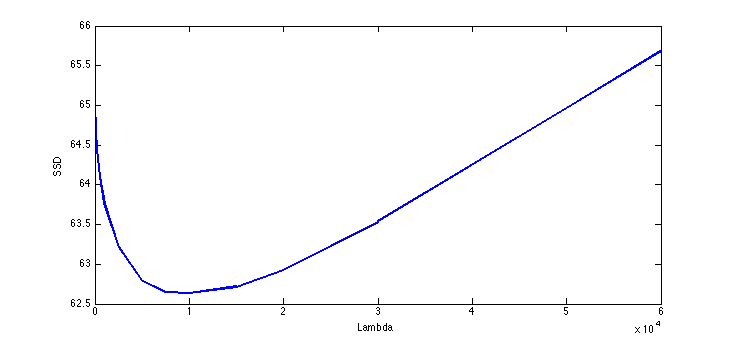
\includegraphics[width=0.9\textwidth]{SSDplot}       
\end{center}
\caption{This figure shows the effect of $\lambda$ on the SSD between the ground-truth $u$ and our solution $\tilde{u}$. The optimal value for $\lambda$ is  approximately 10'000.  }
\label{fig:SSD}
\end{figure}

\item \textbf{ Optimal $\lambda$.} 

Figure \ref{fig:SSD} shows the $\lambda$ vs. SSD graph. We observe that the graph draws a convex function, with a minimum at around 8'000 to 10'000. Similar to the gradient-descent algorithm, very low or high values  for $\lambda$ increase the SSD. For $\lambda=9000$ the primal-dual method obtains a SSD of 62.2. For comparison the gradient-descent method got a SSD of 71.6.


A subjective observation of how the image quality varies with $\lambda$ shows very different behaviour compared to the gradient-descent method. While low values resulted in a "washing out" of image contrast in the gradient method, low $\lambda$ in the primal-dual didn't result in a well-perceivable image degradation. Rather it results in a shift of the image.

\begin{figure}[h]
\begin{center}
         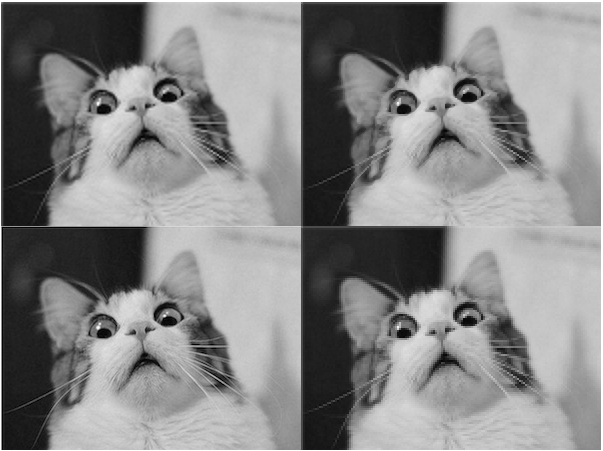
\includegraphics[width=0.9\linewidth]{cat}       
\end{center}
\caption{This figure shows a comparison of the two methods after 1000 iterations. Top-left shows the result of the primal-dual method, top-right gradient descent, bottom-left the ground truth high-res image and bottom-right the low-res input. Computation time: 4.9 sec (primal-dual)  vs. 22.5 sec (gradient). SSD: 71 (primal-dual) vs. 86 (gradient).}
\label{fig:cat}
\end{figure}

\item \textbf{ Conclusions.} 

Figure \ref{fig:cat} shows images comparing the primal-dual and gradient-descent methods. We observe that at the same number of iterations, the computation time and the SSD of the primal-dual method are considerably lower than those of the gradient-descent method. Therefore, the primal-dual method clearly has the better performance of the two. Thanks to variable decoupling it also provides further performance potential as it allows for parallelisation (on a GPU for example). 

\begin{figure}[t]
\begin{center}
\begin{subfigure}[b]{1\textwidth}
                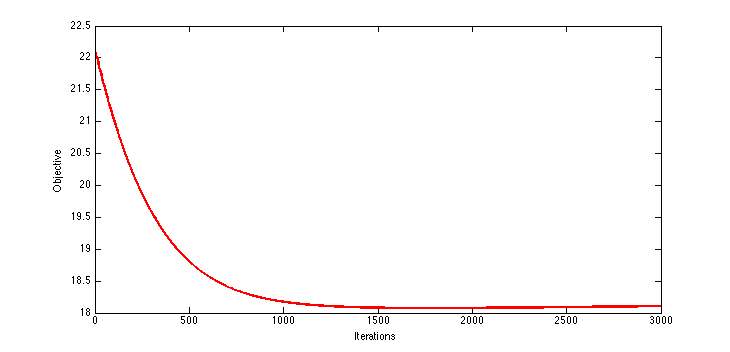
\includegraphics[width=\textwidth]{objective}
                \caption{primal-dual}
        \end{subfigure}
        	\begin{subfigure}[b]{1\textwidth}
                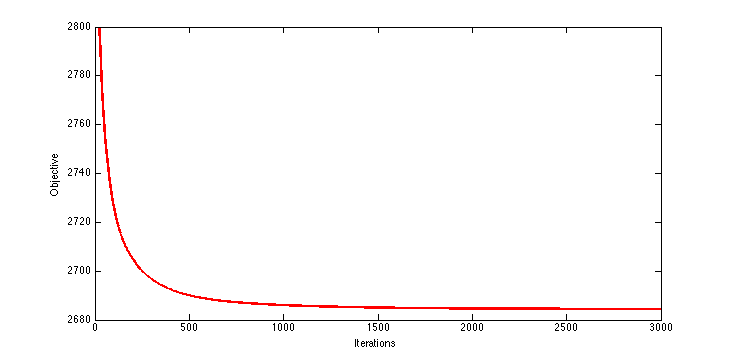
\includegraphics[width=\textwidth]{objGD}
                \caption{gradient-descent}
        \end{subfigure}
\end{center}
\caption{This figure shows the convergence behaviour of the two methods. The upper plot shows the primal-dual objective over time and the lower plot discretised primal objective.}
\label{fig:conv}
\end{figure}

Choosing the parameters for the primal-dual method is not straightforward however and can have a non-negligible effect on the algorithm's performance. Also, the derivation of the steps and the underlying theory are much more involved compared to the gradient-descent method. The convergence behaviour of the two methods is similar, as can be observed in figure \ref{fig:conv}.




\end{enumerate}

 \end{document}
 
 